\section{Tecnologías implementadas y estado operativo.}
\subsection{Análisis de RAM}

Uno de los puntos más importantes a la hora de implementar un bot con IA para un juego de Atari, es entender cómo está hecho. Utilizaremos el entorno \ac{ale} para extraer características de los juegos, el cual cuenta con una API que nos permite extraer información de los mismos. Para ello, se ha desarrollado un lector de RAM que nos ayuda a visualizar los 128 bytes de memoria de la Atari mientras se ejecuta un juego.

Además, dicho lector implementa colores, lo cual permite que se puedan distinguir las posiciones de RAM que cambian de las que no en un step determinado (paso de ejecución)  como se puede ver en la figura \ref{fig:RAM_Colors}.

\begin{figure}[h]
	\centering
	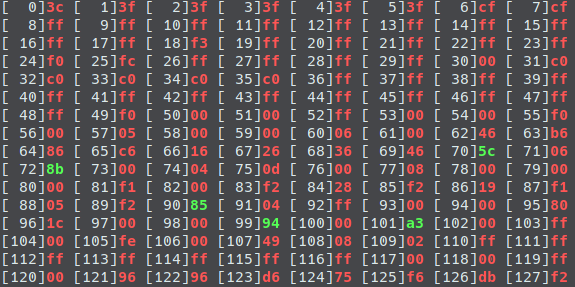
\includegraphics[width=1\textwidth]{Figures/RAMColors}
	\caption{El color verde indica que el valor ha cambiado en este step.}
	\label{fig:RAM_Colors}
\end{figure}

Una de las características de este lector es que acompaña la ejecución con un volcado de analytics para ver las posiciones de RAM que más han cambiado en una ejecución determinada.

Para extraer los datos mas interesantes de un juego en concreto, simplemente hay que observar las posiciones de RAM mas alteradas según nuestro analytics. Una vez hecho esto, se pondrá el juego en cámara lenta gracias a una feature del entorno \ac{ale}, lo cual nos permitirá ver con qué sentido cambian estos valores. Como punto a destacar, no todos los valores que cambian mucho serán relevantes a la hora de sacar datos importantes del juego (un contador podría no ser relevante para un caso específico).

Una vez hecho esto se puede desglosar la RAM de manera bastante precisa, sacando datos como los siguientes.

\begin{figure}[h]
	\centering
	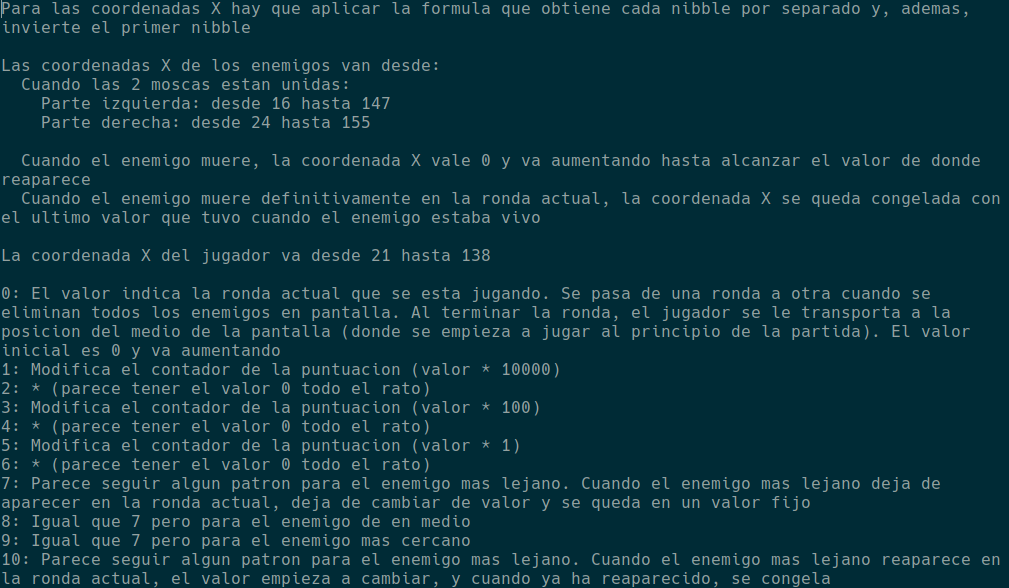
\includegraphics[width=1\textwidth]{Figures/AnalisisRAM}
	\caption{Demon Attack - Análisis de las primeras posiciones de RAM}
	\label{fig:AnalisisRAM}
\end{figure}

Como se puede observar en la figura \ref{fig:AnalisisRAM}, para obtener la información correcta no solo basta con extraer las posiciones relevantes, en algunos casos será necesario procesar esta información. Por ejemplo, en Demon Attack, las coordenadas X de las entidades aparecen obfuscadas de la siguiente manera:

\begin{figure}[h]
	\centering
	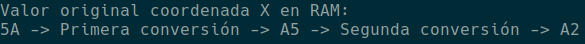
\includegraphics[width=1\textwidth]{Figures/DAttackOpsRequired}
	\caption{Demon Attack - Coordenadas X de las entidades}
	\label{fig:DAttackOpsRequired}
\end{figure}

Como podemos ver en la figura \ref{fig:DAttackOpsRequired}, los nibbles de las coordenadas están invertidos, además, el primer nibble requiere una operacion extra, una resta (7 - valor del nibble). 

Una vez tenemos la información recogida y procesada, la podremos utilizar para crear una IA capaz de jugar al juego en concreto. Además de eso, el entorno \ac{ale} cuenta con diversas funcionalidades que nos permiten recoger la información en pantalla en el caso que fuese necesario. 


\subsection{Bots básicos}


\subsection{Patinete xD}


\newpage